We begin our survey by showing some alarming Sybil attacks happening in the
real-world. Social network and micro-blogging websites are popular platforms for
organisations to improve public relations and their reputation, but they are
also platforms to spread propoganda. A recent article in the Atlantic described
how Twitter bots (Sybils) are shaping the 2016 US presidential
election\cite{atlantictwitterbots}. Over a third of pro-Trump tweets and almost
a fifth of pro-Clinton tweets, totalling at about 1 million, came from bots. The
article questions whether the bots are a threat to democracy because opinions of
real users are eclipsed by the spam of bots.

\begin{figure}
  \centering
  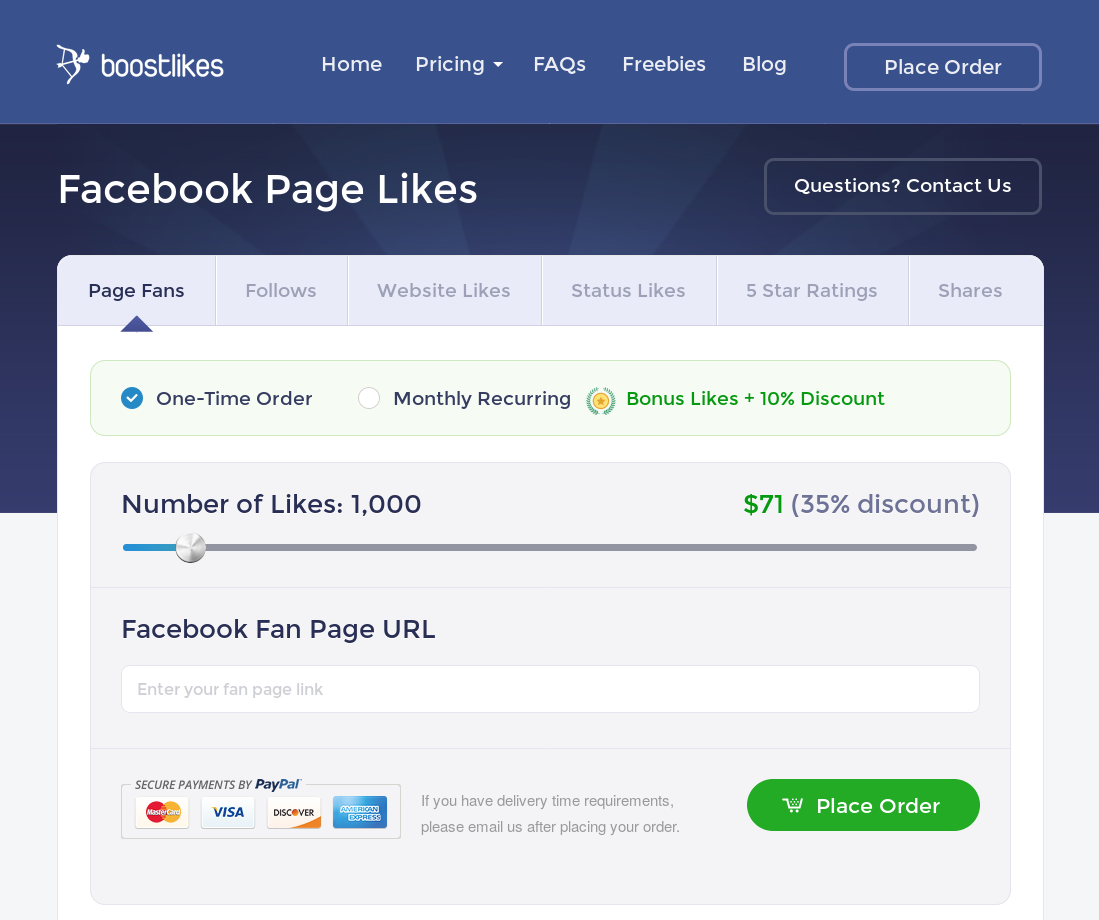
\includegraphics[width=\linewidth]{boostlikes}
  \caption{Screenshot of the Facebook likes service page of boostlikes.com.}
  \label{fig:boostlikes}
\end{figure}

\begin{figure*}
  \centering
  
\includegraphics[width=\textwidth]{socialformulae}
  \caption{Screenshot of the main banner on socialformulae.com.}
  \label{fig:socialformulae}
\end{figure*}

Using Sybils to manipulate public opinion is not only accessible to campaigners
with a large budget. There are marketplaces where anybody can purchase false
reputation scores such as Twitter followers. BoostLikes shown on
\autoref{fig:boostlikes} is a professionally presented website, it offers a
large range of services including Facebook likes, Twitter followers, Instagram
followers and YouTube views\footnote{Facebook is possibly the largest social
  network website at the time of writing. Instagram is a social network website
  designed for sharing photos. YouTube is a video sharing website.}.
SocialFormulae (\autoref{fig:socialformulae}) is a similar service but at a much
lower price point, one thousand Twitter followers is only \$9.99. There can be
little doubt that those companies use automated bots to provide their services.
% one thousand likes cost \$71 at the time of writing. 

SadBotTrue and its related website Socialpuncher publishes studies on social
media fraud. Two of their studies is particularly useful for demonstrating the
scale of the Sybil attack and the obliviousness of Twitter. Firstly, there exist
a botnet that consist of 3 million accounts. Since their creation, they
generated 2.6 billion tweets. Surprisingly, all of the 3 million accounts were
created on the same day---22/10/2013, and the account names are simply
numbered sequentially\cite{sadbottrue}. Such an obvious activity should be
easily detectable by Twitter, but these accounts are still not closed at the
time of writing. Secondly, the top-100 Twitter users have 523 million unique
followers between them, but 310 million are bots, that is almost
60\%\cite{socialpuncher}. Suppose the bots all belong to the same attacker, then
they can effectively suppress the opinions of the real users.

Clearly, the defence mechanisms employed by social network and micro-blogging
websites are not adaquate to combat the Sybil attack. If the Sybils infiltrate
even more of our cyberspace, then it may become a form of censorship.
Effectively taking away our right to freedom of speech.

Speaking of censorship, around a million \cite{tormetric} people use Tor (The
Onion Router)~\cite{dingledine2004tor} to access the uncensored internet when
living in authoritarian regimes such as China, or uphold their privacy from
illegal mass surveillence by intelligence agencies. Unfortunately, Tor suffered
a Sybil attack. In January 2014, 115 bogus relays joined the Tor network. Six months
later, it was discovered that those relays were using a protocol vulnerability
to deanonymise users and find the location of hidden services. It is unclear to
the Tor developers which users are affected or what information was retrieved,
thus it is assumed that users who used Tor between that period are all
affected\cite{torsybil}. In fact, Tor depends on the fact that majority of the
relays are good to guarantee anonymity with a high probability. If the network
is infiltrated by a large number of Sybils then users can be easily
deanonymised.

These example demonstrate a big problem with in the popular social network
websites and anonymous communication tool we use today. A lot of Sybils
controlled by an attacker can censor content and track user behaviour. In the
next section, we zoom in on the practical attacks and grouped them by the
underlying application.

\subsection{Experiment}
We crawled Twitter to gain first-hand knowledge on the real-world sybils.
Twitter was selected because it has an easy-to-use API and it is one of the
major targets of sybils as mentioned at the top of this section.

\subsubsection{Setup}
A Twitter account was created on 25th of November 2016. We purchased the ``1,000
Followers'' product from CoinCrack\footnote{\texttt{coincrack.com}} for \$9. We
made sure our account has 0 tweets and is not advertised in any other medium,
this guarantees that all of its followers are sybils. Followers started coming
in almost immediately after we made our purchase. No more than 1 hour later, our
brand new account with 0 tweets have accumulated 1,300 followers. To find their
relationships, we crawled the followers of sybils for 72 hours using
\verb!tweetf0rm!\footnote{\texttt{https://github.com/bianjiang/tweetf0rm}}
recursively for a depth of three---more than enough for our analysis below.
% We did not crawl 

\subsubsection{Results and Analysis}
We obtained 3 million nodes and 6 million edges by the end of crawling period.
We only consider the known sybils (the followers of our account) for two reasons.
(1) There is no guarantee how many of those 3 million nodes are actually sybils.
(2) Graph visualisation software cannot handle this volume of data under a
reasonable amount of time and computational resources.
% (3) hair-ball
\autoref{fig:twitter-graph} is the result visualised using
Gephi~\cite{bastian2009gephi}. In particular, we use the OpenOrd layout
algorithm~\cite{martin2011openord} to capture the overall structure of the
graph. It structures the layout using hierarchical clustering so that we can
clearly see the communities. We observe the following properties.
\begin{enumerate}
  \item Many sybils are connected with each other, and many of them form a large
    community. This is most likely because the sybils need to be made to look like
    humans so that they can avoid detection. An account that follows thousands of
    users but has 0 followers would look suspicious.
  \item There exist 4 ``super sybils'' (large purple nodes at the centre of the
    graph) and they each have over 1000 followers, so they are connected to
    almost all the other sybils. One of them is
    \verb!@gf1av!\footnote{\texttt{https://twitter.com/gf1av}}, it also joined
    in November 2016 and has over 174K followers at the time of writing. We do
    not know the exact reason for this property, it may be another strategy to
    avoid detection.
  \item The ``1,000 Followers'' service is the cheapest Twitter service, so the
    attacker has many more sybils than what is pictured. Hence the smaller
    communities may be in fact parts of a larger community.
\end{enumerate}

\begin{figure}
  \centering
  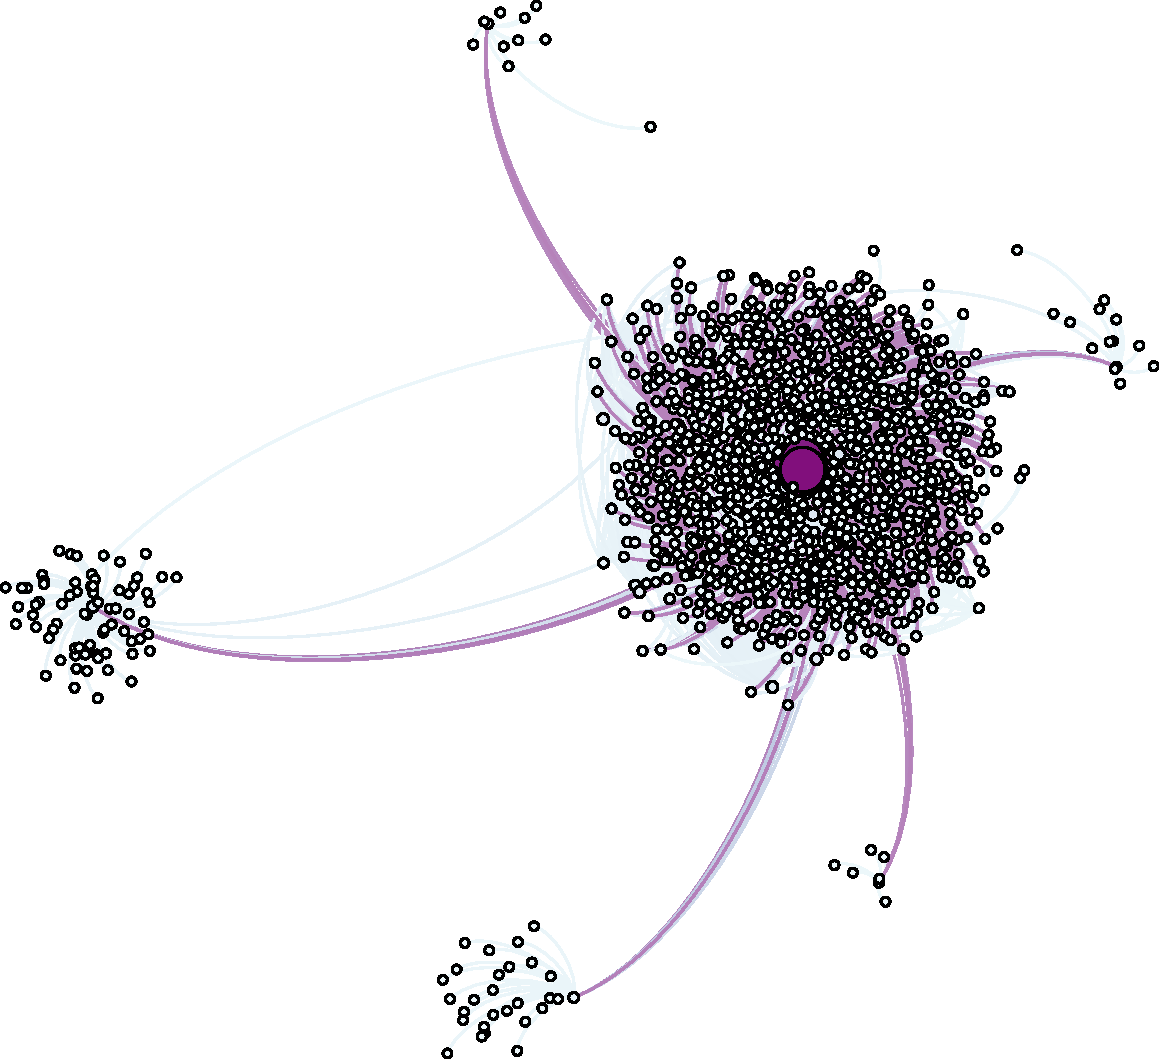
\includegraphics[width=\linewidth]{twitter_graph}
  \caption{Visualisation of the relationships of the sybils. }
  \label{fig:twitter-graph}
\end{figure}

From the results we see the sybils do not have the same characteristics, and
more importantly they form communities within themselves. In
\autoref{sec:defences}, we describe how to leverage the community property to
detect sybils or create sybil-resistant applications.

%%% Local Variables:
%%% mode: latex
%%% TeX-master: "main"
%%% End:
